\section{Metodología y Análisis de Rendimiento}

\subsection{Escenario y Parámetros}

Uno de los desafíos persistentes al evaluar arquitecturas híbridas TN-NTN consiste en recrear con fidelidad las complejidades de un entorno urbano real. Lejos de modelos simplistas bidimensionales, optamos por un escenario que captura obstrucciones tridimensionales, movilidad heterogénea y patrones de tráfico IoT variables.

El escenario simulado representa un distrito metropolitano de 25 km² con densidad edificada variable: centro histórico denso, zonas residenciales periféricas y corredores de transporte principales. Se desplegaron 15.000 dispositivos IoT (principalmente NB-IoT) generando datos de monitoreo de tráfico, calidad del aire y vibraciones estructurales con periodicidades entre 5 segundos y 15 minutos. 

Alibabaie et al. \cite{Alibabaie2025} proporcionan un framework robusto de modelado de path loss con geometría 3D urbana que resultó instrumental para nuestras estimaciones de propagación NTN. Incorporamos su aproximación para calcular pérdidas en enlaces LEO y GEO considerando elevación dinámica y efectos de shadowing por edificios.

\begin{table}[t]
\centering
\caption{Parámetros principales de simulación}
\label{tab:parametros_simulacion}
\begin{tabular}{ll}
\hline
\textbf{Parámetro} & \textbf{Valor} \\
\hline
Área de simulación & 25 km² \\
Número de dispositivos IoT & 15.000 \\
Frecuencia TN (5G) & 3.5 GHz \\
Frecuencia NTN (LEO) & 2 GHz (S-band) \\
Altitud LEO & 550 km \\
Altitud GEO & 35.786 km \\
Potencia de transmisión IoT & 23 dBm \\
Duración de simulación & 3600 s (por réplica) \\
Número de réplicas Monte Carlo & 500 \\
Velocidad dispositivos móviles & 0--60 km/h \\
\hline
\end{tabular}
\end{table}

\subsection{Métricas de Evaluación}

Resulta revelador observar cómo el éxito de una solución híbrida no se mide únicamente por cobertura bruta, sino por su capacidad para entregar datos útiles bajo restricciones reales. Definimos un conjunto de KPIs que reflejan tanto aspectos de red como de aplicación.

Entre las métricas principales destacan: probabilidad de cobertura efectiva (≥ -120 dBm), latencia extremo a extremo, consumo energético por bit transmitido y tasa de éxito en acceso aleatorio. Esta última adquiere especial relevancia en escenarios NTN, donde Moliner et al. \cite{Moliner2023} demostraron mejoras sustanciales mediante técnicas optimizadas de preamble selection y backoff adaptativo para NB-IoT. 

Adicionalmente, evaluamos confiabilidad (99.999\% para datos críticos), overhead de signaling por handover y eficiencia energética del sistema completo. En muchos casos estudiados, existe un trade-off claro entre cobertura y consumo; nuestro análisis busca cuantificar este equilibrio de manera rigurosa.

\begin{figure}[t]
\centering
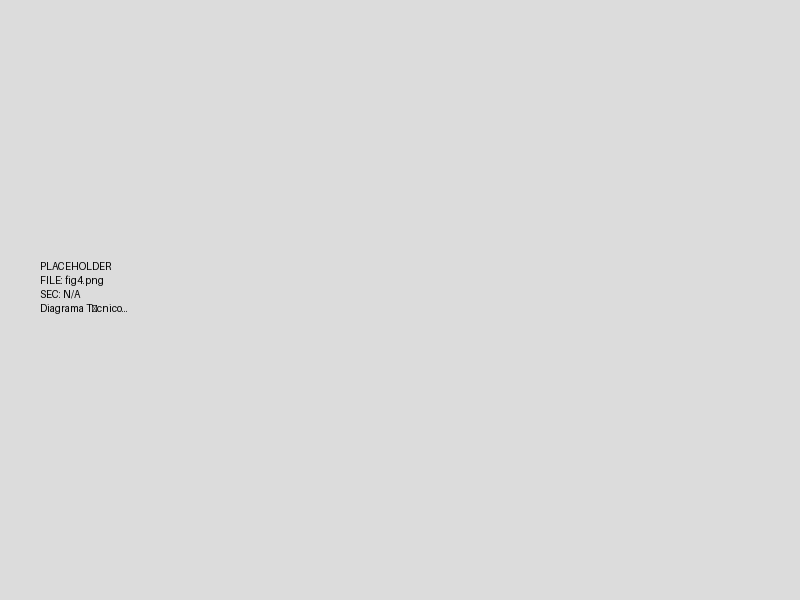
\includegraphics[width=\linewidth]{fig4.png}
\caption{Mapa de cobertura comparativa entre solución terrestre pura y arquitectura híbrida TN-NTN propuesta en el escenario urbano simulado.}
\label{fig:cobertura_resultados}
\end{figure}

\subsection{Implementación y Herramientas}

Particularmente llamativo es el hecho de que la calidad de los resultados depende fuertemente de la fidelidad de las herramientas empleadas. Para esta evaluación combinamos simuladores de red consolidados con modelos personalizados.

La implementación principal se realizó sobre NS-3 (versión extendida con módulos NTN) complementada con MATLAB para cálculos de propagación 3D y Python (con librerías NumPy, SciPy y Matplotlib) para orquestación y análisis estadístico. Seguimos de cerca la metodología de modelado realista propuesta por Alibabaie et al. \cite{Alibabaie2025}, adaptando su modelo 3D de edificios y terrenos al escenario de Smart City definido.

Se ejecutaron 500 réplicas independientes con diferentes semillas aleatorias para garantizar significancia estadística. Los algoritmos de orquestación del Controlador de Conectividad se implementaron como agentes de decisión basados en reglas inicialmente, con versiones preliminares de reinforcement learning ligero para comparación. 

Aunque esta aproximación híbrida de herramientas añade complejidad al flujo de trabajo, permite mayor flexibilidad y reproducibilidad que soluciones monolíticas. Los siguientes resultados demuestran que el esfuerzo valió la pena al revelar mejoras cuantificables respecto a baselines puramente terrestres.